\chapter{Model Predictive Control}\label{chap:background}
\begin{overview}
  With the application of the OI to MPCs shown in the previous chapter, this chapter gives an overview of MPCs in general.
Attention is given to:
\begin{itemize}
  \item general MPC theory,
  \item types of process models used and
  \item how constraints are implemented in MPCs.
\end{itemize}
Finally, background information is presented on two popular commercial MPC packages.
\end{overview}

\section{Model Predictive Control}\label{sec:mpclit}
Since its successful implementation in the petrochemical industry, model predictive control (MPC) has gained widespread acceptance in the processing sector \citep[1]{maciejowskimpc}. 
This has led to the development of many commercial MPC packages such as DMCplus$^{\copyright}$ (Aspentech), RMPCT$^{\copyright}$ (Honeywell), Connoisseur$^{\copyright}$ (Invensys) and SMOC$^{\copyright}$ (Shell Global Solutions) \citep{qinbadgwell}.%
\nomenclature[ba]{DMCPlus}{Dynamic Matrix Control Plus}%
\nomenclature[ba]{RMPCT}{Robust Model Predictive Control Technology}%
\subsection{Nomenclature and notation}
For the sake of coherence between sources a set nomenclature and notation scheme will be used. 
The following variables are defined; $x$ refers to the state of the system, $y$ to the outputs and $u$ to the inputs.
Where vectors are concerned (the MIMO case), a bold face character is used, e.g. $\vect{x}$ for $x$.
Matrices are distinguished by the use of capitals.

The transpose of a matrix or a vector is indicated by a prime ($'$), e.g. $\vect{x}'$.

For discrete time forms, $k$ is used to denote the sample number.
For simplicity of notation, indices are used to refer to samples, i.e. $x_{k+1}$ instead of $x(k+1)$.
\subsection{Control theory}
Model predictive control differs from other model based control techniques (such  as Inverse Nyquist Array- and Internal Model Control) in its active use of predictions for future process outcomes \citep[137]{maciejowskifb}. 
In this context, MPC further distinguishes itself from other predictive control techniques in its ability to accommodate constraints on inputs and outputs.

\citet[8]{maciejowskimpc} summarises the control scheme of MPC in four steps; Measure, Predict, Optimise and Apply. 
These steps are summarized below:
\begin{enumerate}
  \item Measure; the current outputs ($y(t)$) are measured and the error (deviation from the setpoint trajectory, $s(t)$) is calculated.
  \item Predict; using the model, future outputs ($\hat{y}_k$) are calculated (over the prediction horizon, $H_v$).
  \item Optimise (Calculate); control moves (over the control horizon, $H_u$) are now calculated to minimize the predicted deviation from the setpoint trajectory.
  \item Apply; only the first control move is implemented, where-after this procedure is restarted.
\end{enumerate}

Figure~\ref{fig:mpc:general} illustrates the aforementioned steps along with some other responses.
The reference trajectory, $r_k$, shows the ideal response a variable should follow to reach the setpoint trajectory, $s(t)$.
The free response, $\hat{y}_{k~f}$, shows the predicted values of the output if no change to the current control signal is made.

\begin{figure}[htbp]
  \centering
%  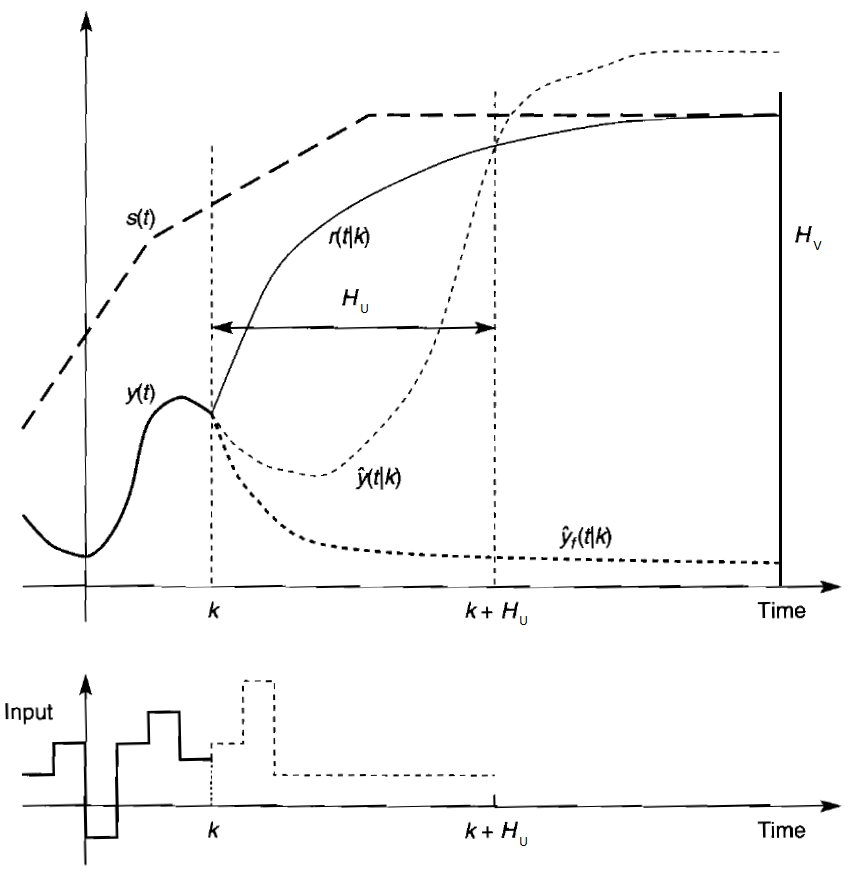
\includegraphics[width=\fullwidth]{graph/mpc_general}
  \scalebox{1}{% Graphic for TeX using PGF
% Title: /home/andre/GIT Repos/AHCampher_thesis/diagrams/mpc_general.dia
% Creator: Dia v0.97.1
% CreationDate: Wed Dec 22 14:43:15 2010
% For: andre
% \usepackage{tikz}
% The following commands are not supported in PSTricks at present
% We define them conditionally, so when they are implemented,
% this pgf file will use them.
\ifx\du\undefined
  \newlength{\du}
\fi
\setlength{\du}{15\unitlength}
\begin{tikzpicture}
\pgftransformxscale{1.000000}
\pgftransformyscale{-1.000000}
\definecolor{dialinecolor}{rgb}{0.000000, 0.000000, 0.000000}
\pgfsetstrokecolor{dialinecolor}
\definecolor{dialinecolor}{rgb}{1.000000, 1.000000, 1.000000}
\pgfsetfillcolor{dialinecolor}
\pgfsetlinewidth{0.100000\du}
\pgfsetdash{}{0pt}
\pgfsetdash{}{0pt}
\pgfsetbuttcap
{
\definecolor{dialinecolor}{rgb}{0.000000, 0.000000, 0.000000}
\pgfsetfillcolor{dialinecolor}
% was here!!!
\pgfsetarrowsend{stealth}
\definecolor{dialinecolor}{rgb}{0.000000, 0.000000, 0.000000}
\pgfsetstrokecolor{dialinecolor}
\draw (2.451747\du,-8.189147\du)--(2.450000\du,-20.440625\du);
}
\pgfsetlinewidth{0.100000\du}
\pgfsetdash{}{0pt}
\pgfsetdash{}{0pt}
\pgfsetbuttcap
{
\definecolor{dialinecolor}{rgb}{0.000000, 0.000000, 0.000000}
\pgfsetfillcolor{dialinecolor}
% was here!!!
\pgfsetarrowsend{stealth}
\definecolor{dialinecolor}{rgb}{0.000000, 0.000000, 0.000000}
\pgfsetstrokecolor{dialinecolor}
\draw (2.425000\du,-8.240625\du)--(29.925000\du,-8.215625\du);
}
\pgfsetlinewidth{0.100000\du}
\pgfsetdash{{\pgflinewidth}{0.200000\du}}{0cm}
\pgfsetdash{{\pgflinewidth}{0.200000\du}}{0cm}
\pgfsetbuttcap
{
\definecolor{dialinecolor}{rgb}{0.000000, 0.000000, 0.000000}
\pgfsetfillcolor{dialinecolor}
% was here!!!
\definecolor{dialinecolor}{rgb}{0.000000, 0.000000, 0.000000}
\pgfsetstrokecolor{dialinecolor}
\draw (7.525000\du,-19.915625\du)--(7.550000\du,-8.265625\du);
}
\pgfsetlinewidth{0.100000\du}
\pgfsetdash{{\pgflinewidth}{0.200000\du}}{0cm}
\pgfsetdash{{\pgflinewidth}{0.200000\du}}{0cm}
\pgfsetbuttcap
{
\definecolor{dialinecolor}{rgb}{0.000000, 0.000000, 0.000000}
\pgfsetfillcolor{dialinecolor}
% was here!!!
\definecolor{dialinecolor}{rgb}{0.000000, 0.000000, 0.000000}
\pgfsetstrokecolor{dialinecolor}
\draw (19.977607\du,-19.923018\du)--(20.002607\du,-8.273018\du);
}
\pgfsetlinewidth{0.100000\du}
\pgfsetdash{{\pgflinewidth}{0.200000\du}}{0cm}
\pgfsetdash{{\pgflinewidth}{0.200000\du}}{0cm}
\pgfsetbuttcap
{
\definecolor{dialinecolor}{rgb}{0.000000, 0.000000, 0.000000}
\pgfsetfillcolor{dialinecolor}
% was here!!!
\definecolor{dialinecolor}{rgb}{0.000000, 0.000000, 0.000000}
\pgfsetstrokecolor{dialinecolor}
\draw (28.480107\du,-19.905518\du)--(28.505107\du,-8.255518\du);
}
\pgfsetlinewidth{0.100000\du}
\pgfsetdash{}{0pt}
\pgfsetdash{}{0pt}
\pgfsetmiterjoin
\pgfsetbuttcap
{
\definecolor{dialinecolor}{rgb}{0.000000, 0.000000, 0.000000}
\pgfsetfillcolor{dialinecolor}
% was here!!!
\definecolor{dialinecolor}{rgb}{0.000000, 0.000000, 0.000000}
\pgfsetstrokecolor{dialinecolor}
\pgfpathmoveto{\pgfpoint{2.511903\du}{-10.002428\du}}
\pgfpathcurveto{\pgfpoint{5.186903\du}{-7.402428\du}}{\pgfpoint{5.111903\du}{-15.152428\du}}{\pgfpoint{7.536903\du}{-13.052428\du}}
\pgfusepath{stroke}
}
\pgfsetlinewidth{0.100000\du}
\pgfsetdash{}{0pt}
\pgfsetdash{}{0pt}
\pgfsetmiterjoin
\pgfsetbuttcap
{
\definecolor{dialinecolor}{rgb}{0.000000, 0.000000, 0.000000}
\pgfsetfillcolor{dialinecolor}
% was here!!!
\definecolor{dialinecolor}{rgb}{0.000000, 0.000000, 0.000000}
\pgfsetstrokecolor{dialinecolor}
\pgfpathmoveto{\pgfpoint{7.511903\du}{-13.052428\du}}
\pgfpathcurveto{\pgfpoint{9.460884\du}{-16.789740\du}}{\pgfpoint{13.786903\du}{-19.152428\du}}{\pgfpoint{28.461903\du}{-19.202428\du}}
\pgfusepath{stroke}
}
\pgfsetlinewidth{0.100000\du}
\pgfsetdash{{1.000000\du}{0.200000\du}{0.200000\du}{0.200000\du}{0.200000\du}{0.200000\du}}{0cm}
\pgfsetdash{{1.000000\du}{0.200000\du}{0.200000\du}{0.200000\du}{0.200000\du}{0.200000\du}}{0cm}
\pgfsetmiterjoin
\pgfsetbuttcap
{
\definecolor{dialinecolor}{rgb}{0.000000, 0.000000, 0.000000}
\pgfsetfillcolor{dialinecolor}
% was here!!!
\definecolor{dialinecolor}{rgb}{0.000000, 0.000000, 0.000000}
\pgfsetstrokecolor{dialinecolor}
\pgfpathmoveto{\pgfpoint{7.513466\du}{-13.066491\du}}
\pgfpathcurveto{\pgfpoint{16.938466\du}{-6.866491\du}}{\pgfpoint{12.586903\du}{-20.477428\du}}{\pgfpoint{28.386903\du}{-20.302428\du}}
\pgfusepath{stroke}
}
\pgfsetlinewidth{0.100000\du}
\pgfsetdash{{1.000000\du}{0.400000\du}{0.200000\du}{0.400000\du}}{0cm}
\pgfsetdash{{1.000000\du}{0.400000\du}{0.200000\du}{0.400000\du}}{0cm}
\pgfsetmiterjoin
\pgfsetbuttcap
{
\definecolor{dialinecolor}{rgb}{0.000000, 0.000000, 0.000000}
\pgfsetfillcolor{dialinecolor}
% was here!!!
\definecolor{dialinecolor}{rgb}{0.000000, 0.000000, 0.000000}
\pgfsetstrokecolor{dialinecolor}
\pgfpathmoveto{\pgfpoint{7.547841\du}{-13.025866\du}}
\pgfpathcurveto{\pgfpoint{9.972841\du}{-8.100866\du}}{\pgfpoint{21.347841\du}{-9.575866\du}}{\pgfpoint{28.397841\du}{-8.750866\du}}
\pgfusepath{stroke}
}
\pgfsetlinewidth{0.100000\du}
\pgfsetdash{{1.000000\du}{1.000000\du}}{0\du}
\pgfsetdash{{1.000000\du}{1.000000\du}}{0\du}
\pgfsetmiterjoin
\pgfsetbuttcap
{
\definecolor{dialinecolor}{rgb}{0.000000, 0.000000, 0.000000}
\pgfsetfillcolor{dialinecolor}
% was here!!!
{\pgfsetcornersarced{\pgfpoint{0.000000\du}{0.000000\du}}\definecolor{dialinecolor}{rgb}{0.000000, 0.000000, 0.000000}
\pgfsetstrokecolor{dialinecolor}
\draw (2.422841\du,-12.700866\du)--(5.222841\du,-16.375866\du)--(15.372841\du,-18.975866\du)--(28.472841\du,-19.175866\du);
}}
\pgfsetlinewidth{0.100000\du}
\pgfsetdash{}{0pt}
\pgfsetdash{}{0pt}
\pgfsetbuttcap
{
\definecolor{dialinecolor}{rgb}{0.000000, 0.000000, 0.000000}
\pgfsetfillcolor{dialinecolor}
% was here!!!
\pgfsetarrowsend{stealth}
\definecolor{dialinecolor}{rgb}{0.000000, 0.000000, 0.000000}
\pgfsetstrokecolor{dialinecolor}
\draw (2.476460\du,-0.012741\du)--(2.470497\du,-7.421085\du);
}
\pgfsetlinewidth{0.100000\du}
\pgfsetdash{}{0pt}
\pgfsetdash{}{0pt}
\pgfsetbuttcap
{
\definecolor{dialinecolor}{rgb}{0.000000, 0.000000, 0.000000}
\pgfsetfillcolor{dialinecolor}
% was here!!!
\pgfsetarrowsend{stealth}
\definecolor{dialinecolor}{rgb}{0.000000, 0.000000, 0.000000}
\pgfsetstrokecolor{dialinecolor}
\draw (2.449713\du,-0.064219\du)--(29.949713\du,-0.039219\du);
}
\pgfsetlinewidth{0.100000\du}
\pgfsetdash{}{0pt}
\pgfsetdash{}{0pt}
\pgfsetmiterjoin
\pgfsetbuttcap
{
\definecolor{dialinecolor}{rgb}{0.000000, 0.000000, 0.000000}
\pgfsetfillcolor{dialinecolor}
% was here!!!
{\pgfsetcornersarced{\pgfpoint{0.000000\du}{0.000000\du}}\definecolor{dialinecolor}{rgb}{0.000000, 0.000000, 0.000000}
\pgfsetstrokecolor{dialinecolor}
\draw (2.476747\du,-1.066302\du)--(3.176747\du,-1.060052\du)--(3.176747\du,-2.972552\du)--(4.014247\du,-2.985052\du)--(4.001747\du,-0.638177\du)--(4.876747\du,-0.638177\du)--(4.876747\du,-3.875677\du)--(5.739247\du,-3.863177\du)--(5.726747\du,-4.513177\du)--(6.539247\du,-4.525677\du)--(6.551747\du,-1.638177\du)--(7.364247\du,-1.625677\du)--(7.351747\du,-4.000677\du)--(7.414247\du,-3.988177\du);
}}
\pgfsetlinewidth{0.100000\du}
\pgfsetdash{{1.000000\du}{1.000000\du}}{0\du}
\pgfsetdash{{0.500000\du}{0.500000\du}}{0\du}
\pgfsetmiterjoin
\pgfsetbuttcap
{
\definecolor{dialinecolor}{rgb}{0.000000, 0.000000, 0.000000}
\pgfsetfillcolor{dialinecolor}
% was here!!!
{\pgfsetcornersarced{\pgfpoint{0.000000\du}{0.000000\du}}\definecolor{dialinecolor}{rgb}{0.000000, 0.000000, 0.000000}
\pgfsetstrokecolor{dialinecolor}
\draw (20.095497\du,-0.808490\du)--(10.523622\du,-0.867865\du)--(10.504872\du,-3.005365\du)--(9.517372\du,-3.005365\du)--(9.511122\du,-1.011615\du)--(8.486122\du,-1.017865\du)--(8.486122\du,-4.025677\du)--(7.354872\du,-4.019427\du);
}}
% setfont left to latex
\definecolor{dialinecolor}{rgb}{0.000000, 0.000000, 0.000000}
\pgfsetstrokecolor{dialinecolor}
\node[anchor=west] at (14.650069\du,-6.745990\du){Time};
% setfont left to latex
\definecolor{dialinecolor}{rgb}{0.000000, 0.000000, 0.000000}
\pgfsetstrokecolor{dialinecolor}
\node[anchor=west] at (14.665784\du,1.629010\du){Time};
% setfont left to latex
\definecolor{dialinecolor}{rgb}{0.000000, 0.000000, 0.000000}
\pgfsetstrokecolor{dialinecolor}
\node[anchor=west] at (7.363284\du,-7.433490\du){$k$};
% setfont left to latex
\definecolor{dialinecolor}{rgb}{0.000000, 0.000000, 0.000000}
\pgfsetstrokecolor{dialinecolor}
\node[anchor=west] at (18.988284\du,-7.458490\du){$k+H_u$};
% setfont left to latex
\definecolor{dialinecolor}{rgb}{0.000000, 0.000000, 0.000000}
\pgfsetstrokecolor{dialinecolor}
\node[anchor=west] at (7.315784\du,0.704010\du){$k$};
% setfont left to latex
\definecolor{dialinecolor}{rgb}{0.000000, 0.000000, 0.000000}
\pgfsetstrokecolor{dialinecolor}
\node[anchor=west] at (18.965784\du,0.729010\du){$k+H_u$};
% setfont left to latex
\definecolor{dialinecolor}{rgb}{0.000000, 0.000000, 0.000000}
\pgfsetstrokecolor{dialinecolor}
\node[anchor=west] at (28.163284\du,-7.258490\du){$H_v$};
% setfont left to latex
\definecolor{dialinecolor}{rgb}{0.000000, 0.000000, 0.000000}
\pgfsetstrokecolor{dialinecolor}
\node[anchor=west] at (-0.674216\du,-13.989740\du){Output};
% setfont left to latex
\definecolor{dialinecolor}{rgb}{0.000000, 0.000000, 0.000000}
\pgfsetstrokecolor{dialinecolor}
\node[anchor=west] at (0.000784\du,-3.495990\du){Input};
% setfont left to latex
\definecolor{dialinecolor}{rgb}{0.000000, 0.000000, 0.000000}
\pgfsetstrokecolor{dialinecolor}
\node[anchor=west] at (4.460884\du,-17.014740\du){$s(t)$};
% setfont left to latex
\definecolor{dialinecolor}{rgb}{0.000000, 0.000000, 0.000000}
\pgfsetstrokecolor{dialinecolor}
\node[anchor=west] at (10.260884\du,-15.489740\du){$r_k$};
% setfont left to latex
\definecolor{dialinecolor}{rgb}{0.000000, 0.000000, 0.000000}
\pgfsetstrokecolor{dialinecolor}
\node[anchor=west] at (3.160884\du,-11.039740\du){$y(t)$};
% setfont left to latex
\definecolor{dialinecolor}{rgb}{0.000000, 0.000000, 0.000000}
\pgfsetstrokecolor{dialinecolor}
\node[anchor=west] at (15.385884\du,-13.189740\du){$\hat{y}_k$};
% setfont left to latex
\definecolor{dialinecolor}{rgb}{0.000000, 0.000000, 0.000000}
\pgfsetstrokecolor{dialinecolor}
\node[anchor=west] at (23.138384\du,-9.627240\du){$\hat{y}_{f~k}$};
\end{tikzpicture}
}  
  \caption[General MPC working]{General MPC working, showing predictions on both outputs and inputs \citep[8]{maciejowskimpc}}
  \label{fig:mpc:general}
\end{figure}

\subsection{Objective functions}
Optimal control moves are defined in terms of objective functions.
These functions are often referred to as cost functions \citep[41]{maciejowskimpc} as they can incorporate input and output weighting based on economic factors.

The general formulation of the unconstrained objective function is presented in equation~\ref{eq:genobjfn}. 
Modifications to this function (due to constraints) is discussed in section~\ref{sec:conobjfn}. 
From \citet[17]{rawlings} and \citet[41]{maciejowskimpc}, the objective function which penalizes deviations from the setpoint trajectory as well as moves in the inputs is shown below;
% TODO - eqn in terms of zero setpoint, generalize to non-zero sp
\begin{equation}
  \label{eq:genobjfn}
  V(\vect{x}_0,\vect{u})=\frac{1}{2}\sum^{N-1}_{k=0}[\vect{x}_k'Q\vect{x}_k + \vect{u}_k'R\vect{u}_k]
  + \frac{1}{2}\vect{x}_N'P_f\vect{x}_N
\end{equation}
It is clear that the objective function depends on both the state sequence and the input sequence. 
The current state, $\vect{x}_0$ is known (measured) and the subsequent states are determined by the model and the input sequence. 
The optimal MPC control problem therefore becomes;
\begin{equation}
  \label{eq:opctrlprob}
  \min_{\vect{u}} V(\vect{x}_0,{\bf u})
\end{equation}

\subsection{Models}
The correct choice of model is one of the most important steps in the operation of MPCs \citep[17]{rossiter}.
This is due to the active use of the model in making predictions as the controller runs, and not serving merely as an analysis aid \citep[37]{maciejowskimpc}.

\subsubsection{State space models}
State space models are the most encountered type in literature.
The general, linear, time-variant, state space model is presented in equation~\ref{eq:genss}.
\begin{align}
  \label{eq:genss}
  \ddfrac{\vect{x}}{t} &= A(t)\vect{x} + B(t)\vect{u} \notag \\
  \vect{y} &= C(t)\vect{x} + D(t)\vect{u} \\
  \vect{x}(0) &= \vect{x}_0 \notag
\end{align}
Where $A(t),~B(t),~C(t)$ and $D(t)$ are appropriately sized matrices of the state space model, and $\vect{x}_0$ is the initial state of the system.
For the time-invariant case, these matrices simply reduce to $A,~B,~C$ and $D$. 
As MPC is mostly implemented at discrete time steps, the model in equation~\ref{eq:genss} (for the time-invariant case) translates to equation~\ref{eq:genssdisc}.
\begin{align}
  \label{eq:genssdisc}
  \vect{x}_{k+1} &= A\vect{x}_k + B\vect{u}_k \notag \\
  \vect{y}_k &= C\vect{x}_k + D\vect{u}_k \\
  \vect{x}_0 &~ \text{(given)} \notag
\end{align}

\subsubsection{Step and pulse response models}
Step and pulse response models, especially finite impulse response (FIR) models, were widely used in the original descriptions of MPC.
There has, however, been a recent trend to move to other model types, such as transfer function models \citepp{113}{maciejowskimpc}{26}{rossiter}.

The pulse response model can be defined using the common convolution model \citep[284]{luyben}, as shown in equation~\ref{eq:fir}.
Where $H$ is a matrix representing the response of an output to a unit pulse in the corresponding input.
\begin{equation}
  \label{eq:fir}
  \vect{y}(t) = \sum^t_{k=0}H(t-k)\vect{u}_k
\end{equation} 
Even though FIR models are intuitive they are not without shortcomings.
The most prominent of these problems are that FIR models are only applicable to asymptotically stable plants, and they are only adequate if the CVs are measured outputs.
\citet[109]{maciejowskimpc} elaborates on this topic.

\subsubsection{Transfer function models}
In the Laplace domain, the input to output relationship of a generic process (as shown in figure~\ref{fig:genmodel}) is represented by;
\begin{equation*}
  \vect{\bar y}(s)=G(s)\vect{\bar u}(s)
\end{equation*}
where $G$ is the process matrix, and $\vect{\bar u}$ and $\vect{\bar y}$ are the process inputs and outputs (with the bars indicating deviation variables) respectively.
The process matrix ($G$) can contain dynamic elements or, in the case of a steady-state model, only gains.
Note that state ($\vect{x}$) information does not appear in the transfer function formulation.
\begin{figure}[htbp]
  \centering
%  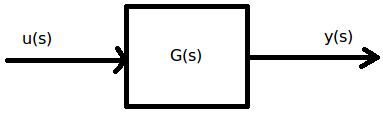
\includegraphics[width=8cm]{graph/model_genprocess}
  \scalebox{1}{% Graphic for TeX using PGF
% Title: /home/andre/GIT Repos/AHCampher_thesis/diagrams/model_genprocess.dia
% Creator: Dia v0.97.1
% CreationDate: Fri Dec 24 11:34:12 2010
% For: andre
% \usepackage{tikz}
% The following commands are not supported in PSTricks at present
% We define them conditionally, so when they are implemented,
% this pgf file will use them.
\ifx\du\undefined
  \newlength{\du}
\fi
\setlength{\du}{15\unitlength}
\begin{tikzpicture}
\pgftransformxscale{1.000000}
\pgftransformyscale{-1.000000}
\definecolor{dialinecolor}{rgb}{0.000000, 0.000000, 0.000000}
\pgfsetstrokecolor{dialinecolor}
\definecolor{dialinecolor}{rgb}{1.000000, 1.000000, 1.000000}
\pgfsetfillcolor{dialinecolor}
\pgfsetlinewidth{0.100000\du}
\pgfsetdash{}{0pt}
\pgfsetdash{}{0pt}
\pgfsetmiterjoin
\definecolor{dialinecolor}{rgb}{1.000000, 1.000000, 1.000000}
\pgfsetfillcolor{dialinecolor}
\fill (12.462700\du,7.562500\du)--(12.462700\du,10.087500\du)--(17.387700\du,10.087500\du)--(17.387700\du,7.562500\du)--cycle;
\definecolor{dialinecolor}{rgb}{0.000000, 0.000000, 0.000000}
\pgfsetstrokecolor{dialinecolor}
\draw (12.462700\du,7.562500\du)--(12.462700\du,10.087500\du)--(17.387700\du,10.087500\du)--(17.387700\du,7.562500\du)--cycle;
% setfont left to latex
\definecolor{dialinecolor}{rgb}{0.000000, 0.000000, 0.000000}
\pgfsetstrokecolor{dialinecolor}
\node[anchor=west] at (13.825200\du,8.875000\du){$G(s)$};
\pgfsetlinewidth{0.100000\du}
\pgfsetdash{}{0pt}
\pgfsetdash{}{0pt}
\pgfsetbuttcap
{
\definecolor{dialinecolor}{rgb}{0.000000, 0.000000, 0.000000}
\pgfsetfillcolor{dialinecolor}
% was here!!!
\pgfsetarrowsend{stealth}
\definecolor{dialinecolor}{rgb}{0.000000, 0.000000, 0.000000}
\pgfsetstrokecolor{dialinecolor}
\draw (6.837700\du,8.862500\du)--(12.462700\du,8.825000\du);
}
\pgfsetlinewidth{0.100000\du}
\pgfsetdash{}{0pt}
\pgfsetdash{}{0pt}
\pgfsetbuttcap
{
\definecolor{dialinecolor}{rgb}{0.000000, 0.000000, 0.000000}
\pgfsetfillcolor{dialinecolor}
% was here!!!
\pgfsetarrowsend{stealth}
\definecolor{dialinecolor}{rgb}{0.000000, 0.000000, 0.000000}
\pgfsetstrokecolor{dialinecolor}
\draw (17.387700\du,8.825000\du)--(23.412700\du,8.837500\du);
}
% setfont left to latex
\definecolor{dialinecolor}{rgb}{0.000000, 0.000000, 0.000000}
\pgfsetstrokecolor{dialinecolor}
\node[anchor=west] at (6.112700\du,8.162500\du){$\vect{\bar{u}}(s)$};
% setfont left to latex
\definecolor{dialinecolor}{rgb}{0.000000, 0.000000, 0.000000}
\pgfsetstrokecolor{dialinecolor}
\node[anchor=west] at (21.985200\du,8.087500\du){$\vect{\bar{y}}(s)$};
\end{tikzpicture}
}
  \caption[Generic input to output model]{Generic process showing inputs ($\vect{\bar y}$), model ($G$) and outputs ($\vect{\bar x}$).}
  \label{fig:genmodel}
\end{figure}

With the assumption of an initial zero state ($\vect{x}_0=0$), the state space description can be converted to a transfer function description.
Taking the Laplace transform of equation~\ref{eq:genss} (for the time-invariant case), and rearranging, results in equation~\ref{eq:gentf}.
\begin{align}
  \label{eq:gentf}
    \vect{\bar x}(s) &= (sI-A)^{-1}B\vect{\bar u}(s) \\
    \vect{\bar y}(s) &= (C(sI-A)^{-1}B+D)\vect{\bar u}(s) \notag
\end{align} 
\subsubsection{Other model types}
Some other model types are also used in MPCs, most are however derived from or reformulations of the above mentioned types.
Examples include, distributed models \citep[4]{rawlings}, CARIMA models and matrix fraction descriptions \citep[24,28]{rossiter} -- with the later two stemming from transfer function descriptions.

Even though only linear models have been presented in this section, many MPCs are capable of using non-linear models.
The use of linear models in MPC is, however, common practice.
Important reasons for this are; no assurance of convergence of solutions and optimisation being non-trivial for non-linear models \citep[17]{rossiter}.

\subsection{Tuning}
The tuning of MPCs is a complex task with many adjustable parameters, even in basic formulations.
Most tuning is, however, based on experience or rules of thumb \citep[188]{maciejowskimpc}.

As far as the objective function (equation~\ref{eq:genobjfn}) is concerned, the most prominent tuning parameters for MPCs are the weighting matrices $Q$, $R$ and $P_f$. 
These are used to enforce the relative importance of deviations in both the inputs and outputs.

The weighting matrices are by no means the only tuning parameters.
Additional parameters include the horizons used for predictions, the reference trajectory and the auxiliary models used (e.g. disturbance models). 
Chapter 7 of \citet{maciejowskimpc} covers the tuning of MPCs in some detail.

\section{Constraints in MPC}
The implementation of constraints is probably the most important selling point of MPCs.
When used in conjunction with a steady-state optimiser, MPCs are able to operate with more CVs than MVs \citep{vinsonphd}. 
When this is the case, additional degrees of freedom are obtained by controlling CVs within ranges rather than on setpoints.

\subsection{Constraint types}
Different types of constraints are present in the MPC algorithm.
The following section lists these constraints and give a short description of their function and properties.
\subsubsection{Control constraints}
Often called ``hard'' constraints, these constraints are used for control (as opposed to optimisation) and are never violated when control moves are calculated.
Control constraints exist for both outputs and inputs, and typically sort into two categories:
\begin{itemize}
  \item The constraints on inputs are typically physical constraints.
    Examples are valve saturation limits and maximum heat duties.
    Control constraints on outputs are usually concerned with safety and damage to equipment.
    Tank levels are an example of this.
  \item Another class of control constraints (usually on outputs) are concerned with product quality and are thus operational in nature.
\end{itemize}
To add robustness to the control solution, some commercial MPCs use constraints that regulate dynamic behaviour.
These are typically a changing constraint at each solution interval.
Examples of these so called ``funnels'' are given in section~\ref{sec:rmpctcons}.

\subsubsection{Optimisation constraints}
The constraints implemented by the optimisers in MPC are often called ``soft'' constraints.
These constraints are typically determined by operational and economical factors.
These constraints are usually implemented as steady-state constraints which represent the optimal solutions of an external cost function.
The limits of these constraints are contained within the control constraints mentioned above.

As these constraints are not determined by the control objective function, situations exist where they are violated in an attempt to ensure feasibility of the MPC solution.
This is discussed further in section~\ref{sec:coneffsol}.
 
\subsection{Constraint formulation}
Constraints on the inputs, outputs or states of a system can be represented as sets of linear inequalities.
For the most general case, they can be expressed as follows:
\begin{align}
  \label{eq:gencons}
  A_u\vect{u}_k &\leq \vect{b}_u \notag \\
  A_y\vect{y}_k &\leq \vect{b}_y \\
  A_x\vect{x}_k &\leq \vect{b}_x \notag
\end{align}
where $A_u,~A_y$ and $A_x$ are coefficient matrices, and $\vect{b}_u,~\vect{b}_y$ and $\vect{b}_x$ the half-space offsets.
For the case where only upper and lower bounds on variables exist, $A_u$ and $\vect{b}_u$ reduce to:%
\nomenclature[a]{$A$}{Coefficient matrix for constraints (used with subscript)}%
\nomenclature[a]{$b$}{half-space offsets for constraints (used with subscript)}%

\begin{align*}
  A_u={I\brack -I} \qquad \vect{b}_u={\vect{u}^{max}_k \brack -\vect{u}^{min}_k}
\end{align*}
where $\vect{u}^{max}_k$ and $\vect{u}^{min}_k$ correspond to the upper and lower limits of $\vect{u}_k$ respectively \citep[6]{rawlings}. 
The coefficient matrices and offsets are reduced similarly for the outputs and the states.

For constraints on rate of change of inputs, the formulation is similar to equation~\ref{eq:gencons}.
The change in $\vect{u}_k$ during a sampling instance is now considered thus:
\begin{align*}
  A_{\Delta u}\Delta \vect{u}_k &\leq \vect{b}_{\Delta u} \notag \\
  \text{with}~~ \Delta \vect{u}_k &= \vect{u}_{k+1}-\vect{u}_k
\end{align*}

\subsection{Quadratic objective functions}\label{sec:conobjfn}
When constraints are present, the general objective function (equation~\ref{eq:genobjfn}), now subject to equation~\ref{eq:gencons} can be reformulated as a quadratic programming (QP) problem.
This makes the problem convex and has favourable consequences for the solution of the optimisation.

The mathematical description of the QP problem is omitted from this dissertation.
\citet[81-83]{maciejowskimpc} as well as \citet[489-490]{rawlings} can be consulted for the complete reformulation.

\subsection{Effect on solutions}\label{sec:coneffsol}
The reformulation of the objective function and constraints into a QP problem -- and the subsequent convexity of the optimisation -- affects the solution in numerous ways.
\citet[83]{maciejowskimpc} lists some of the solution properties obtained; namely that the termination of the QP problem is guaranteed and that computation time can be calculated.

Constrained optimisation does however suffer from the problem of possible infeasibilities. 
For commercial MPCs the solvers are usually custom built to provide a ``back-up'' solution in the case of infeasibilities.
This back-up solution usually consists of modifying constraints (hence the term ``constraint handling'').
The most common methods of internal constraint handling are listed below:
\begin{itemize}
\item Constraint softening, where constraints are prioritized and then relaxed (or removed) until feasibility is obtained \citep[160]{rossiter}.
\item Using constraint windows which define a horizon over which constraints are enforced.
Feasibility can now be obtained by changing the start and end-time of this window \citep[281-282]{maciejowskimpc}.
\item Back- offs and borders can be defined, effectively changing all constraints into ``soft'' constraints.
Due to the conservative approach, setting the back -off amounts therefore becomes a feasibility assurance and performance compromise \citepp{161}{rossiter}{282}{maciejowskimpc}.
\end{itemize}


\section{Commercial MPCs}\label{sec:commercialmpc}
This section gives a more detailed overview of two popular commercial MPC packages.
Appendix~\ref{app:screenshots} contains screenshots of the interfaces mentioned in the sections that follow.

\subsection{Honeywell RMPCT}
Honeywell's MPC controller, RMPCT (Robust Model Predictive Control Technology), forms part of their advanced process control suite, Profit Suite.
A brief overview of the controller and optimiser is given below. 
Attention is given to the controller internals as well as the interface used to build such a controller.
The information presented in this section is taken from \citet{honeywell1}, \citet{honeywell2} and \citet{honeywell3} unless stated otherwise.

\subsubsection{Models}
For the purpose of predictions, process models usually need to be identified first -- typically via step testing.
\citet{honeywell3} lists the types of models which are supported by their Identifier and elaborates on their specific application.
These model types include:
\begin{itemize}
\item FIR,
\item PEM (the structure of which supports FIR, ARX, ARMA, ARMAX, ARIMA(X), ARARMAX, BJ and OE models) and
\item Laplace domain parametric models.
\end{itemize}
The final model, however, is saved in the Laplace domain.
Discrete models are converted to the {\it s} domain and has a final structure as shown in equation~\ref{eq:rmpctmodel}.
\begin{equation}
  \label{eq:rmpctmodel}
  G(s) = \frac{k(b_{n-1}s^{n-1}+ \cdots b_1s+1)e^{-ds}} {s(a_ns^n+a_{n-1}s^{n-1}+ \cdots a_1s+1)}
\end{equation}
The leading {\it s} in the denominator of equation~\ref{eq:rmpctmodel} indicates an integrator in any of the sub-processes.

If a third-party model exists, then the model converter in Profit Suite can be used to convert it into a suitable form.
  
\subsubsection{Constraints}\label{sec:rmpctcons}
For MVs, the implementation of control constraints are in the form of high and low limits, and movement limits.
The high and low limits of MVs are never violated.
Prioritisation and move suppression of MVs are done by means of weighting factors.
The movement load ($L_{\Delta}$) is spread across the MVs as per equation~\ref{eq:rmpctmvload}.
\begin{equation}
  \label{eq:rmpctmvload}
  L_{\Delta} = \min \sum_j \Delta u_j^2 \times w_j^2
\end{equation}
where $w$ is the weight and $j$ the index of the MV.

CV control constraints are also specified as high and low limits.
In the event of negative degrees of freedom, constraints are prioritised by means of a give-up factor called the engineering unit (EU) give up.
Similar to equation~\ref{eq:rmpctmvload} the cumulative weighted error on the CVs ($\epsilon$) is minimised as per equation~\ref{eq:rmpctcverror} with the weight ($w$) defined as shown.
\begin{align}
  \label{eq:rmpctcverror}
  \epsilon = \min \sum_i w_i^2 \times e_i^2 \\
  w = \frac{1}{(\text{CV scaling factor})_i\sqrt{(\text{EU give up})_i}} \notag
\end{align}
where $e$ is the error and $i$ the CV index

The optimisation constraints are defined as being a specified amount within the high or low control limits.
These limits are not used for control.

For the constraining of dynamic response, funnels are implemented.
Predefined funnel types can be chosen from:
\begin{itemize}
\item Type 0, which is an automatically generated funnel,
\item Type 1, defined as a third of the Type 0 funnel pinched using the feedback performance ratio (FPR), and
\item Type 2, which is similar to Type 1 but pinched with the decouple ratio (Type 2 is therefore FPR independent).
\end{itemize}
Figure~\ref{fig:rmpctfunnel} illustrates the concept of pinching for the RMPCT funnels.
The definitions of the FPR and the decouple ratio are contained in \citet{honeywell1} but are omitted from this dissertation.
\begin{figure}[htbp]
  \centering
%  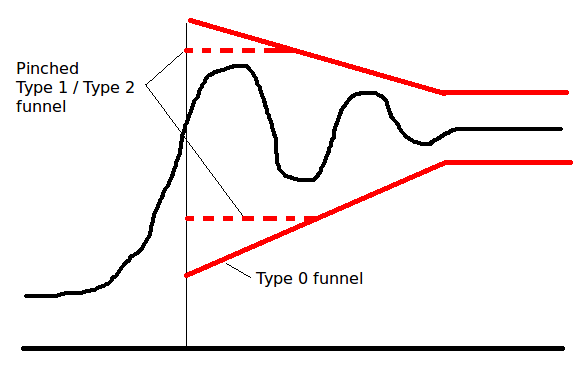
\includegraphics[width=\fullwidth]{rmpct_funnel}
  \scalebox{1}{% Graphic for TeX using PGF
% Title: /home/andre/GIT Repos/AHCampher_thesis/diagrams/rmpctfunnel.dia
% Creator: Dia v0.97.1
% CreationDate: Thu Jan  6 16:11:33 2011
% For: andre
% \usepackage{tikz}
% The following commands are not supported in PSTricks at present
% We define them conditionally, so when they are implemented,
% this pgf file will use them.
\ifx\du\undefined
  \newlength{\du}
\fi
\setlength{\du}{15\unitlength}
\begin{tikzpicture}
\pgftransformxscale{1.000000}
\pgftransformyscale{-1.000000}
\definecolor{dialinecolor}{rgb}{0.000000, 0.000000, 0.000000}
\pgfsetstrokecolor{dialinecolor}
\definecolor{dialinecolor}{rgb}{1.000000, 1.000000, 1.000000}
\pgfsetfillcolor{dialinecolor}
\pgfsetlinewidth{0.050000\du}
\pgfsetdash{}{0pt}
\pgfsetdash{}{0pt}
\pgfsetbuttcap
{
\definecolor{dialinecolor}{rgb}{0.000000, 0.000000, 0.000000}
\pgfsetfillcolor{dialinecolor}
% was here!!!
\definecolor{dialinecolor}{rgb}{0.000000, 0.000000, 0.000000}
\pgfsetstrokecolor{dialinecolor}
\draw (10.000000\du,15.000000\du)--(33.000000\du,15.000000\du);
}
\pgfsetlinewidth{0.050000\du}
\pgfsetdash{}{0pt}
\pgfsetdash{}{0pt}
\pgfsetbuttcap
{
\definecolor{dialinecolor}{rgb}{0.000000, 0.000000, 0.000000}
\pgfsetfillcolor{dialinecolor}
% was here!!!
\definecolor{dialinecolor}{rgb}{0.000000, 0.000000, 0.000000}
\pgfsetstrokecolor{dialinecolor}
\draw (16.000000\du,3.000000\du)--(16.000000\du,15.000000\du);
}
\pgfsetlinewidth{0.150000\du}
\pgfsetdash{}{0pt}
\pgfsetdash{}{0pt}
\pgfsetbuttcap
{
\definecolor{dialinecolor}{rgb}{0.588235, 0.588235, 0.588235}
\pgfsetfillcolor{dialinecolor}
% was here!!!
\definecolor{dialinecolor}{rgb}{0.588235, 0.588235, 0.588235}
\pgfsetstrokecolor{dialinecolor}
\draw (33.000000\du,7.000000\du)--(27.000000\du,7.000000\du);
}
\pgfsetlinewidth{0.150000\du}
\pgfsetdash{}{0pt}
\pgfsetdash{}{0pt}
\pgfsetbuttcap
{
\definecolor{dialinecolor}{rgb}{0.588235, 0.588235, 0.588235}
\pgfsetfillcolor{dialinecolor}
% was here!!!
\definecolor{dialinecolor}{rgb}{0.588235, 0.588235, 0.588235}
\pgfsetstrokecolor{dialinecolor}
\draw (33.000000\du,10.000000\du)--(27.000000\du,10.000000\du);
}
\pgfsetlinewidth{0.150000\du}
\pgfsetdash{}{0pt}
\pgfsetdash{}{0pt}
\pgfsetbuttcap
{
\definecolor{dialinecolor}{rgb}{0.588235, 0.588235, 0.588235}
\pgfsetfillcolor{dialinecolor}
% was here!!!
\definecolor{dialinecolor}{rgb}{0.588235, 0.588235, 0.588235}
\pgfsetstrokecolor{dialinecolor}
\draw (27.000000\du,7.000000\du)--(16.000000\du,3.000000\du);
}
\pgfsetlinewidth{0.150000\du}
\pgfsetdash{}{0pt}
\pgfsetdash{}{0pt}
\pgfsetbuttcap
{
\definecolor{dialinecolor}{rgb}{0.588235, 0.588235, 0.588235}
\pgfsetfillcolor{dialinecolor}
% was here!!!
\definecolor{dialinecolor}{rgb}{0.588235, 0.588235, 0.588235}
\pgfsetstrokecolor{dialinecolor}
\draw (27.000000\du,10.000000\du)--(16.000000\du,12.000000\du);
}
\pgfsetlinewidth{0.150000\du}
\pgfsetdash{{0.700000\du}{0.700000\du}}{0\du}
\pgfsetdash{{0.500000\du}{0.500000\du}}{0\du}
\pgfsetbuttcap
{
\definecolor{dialinecolor}{rgb}{0.000000, 0.000000, 0.000000}
\pgfsetfillcolor{dialinecolor}
% was here!!!
\definecolor{dialinecolor}{rgb}{0.000000, 0.000000, 0.000000}
\pgfsetstrokecolor{dialinecolor}
\draw (16.000000\du,5.000000\du)--(21.500000\du,5.000000\du);
}
\pgfsetlinewidth{0.150000\du}
\pgfsetdash{{0.500000\du}{0.500000\du}}{0\du}
\pgfsetdash{{0.500000\du}{0.500000\du}}{0\du}
\pgfsetbuttcap
{
\definecolor{dialinecolor}{rgb}{0.000000, 0.000000, 0.000000}
\pgfsetfillcolor{dialinecolor}
% was here!!!
\definecolor{dialinecolor}{rgb}{0.000000, 0.000000, 0.000000}
\pgfsetstrokecolor{dialinecolor}
\draw (16.000000\du,11.000000\du)--(21.500000\du,11.000000\du);
}
\pgfsetlinewidth{0.100000\du}
\pgfsetdash{}{0pt}
\pgfsetdash{}{0pt}
\pgfsetmiterjoin
\pgfsetbuttcap
{
\definecolor{dialinecolor}{rgb}{0.000000, 0.000000, 0.000000}
\pgfsetfillcolor{dialinecolor}
% was here!!!
\definecolor{dialinecolor}{rgb}{0.000000, 0.000000, 0.000000}
\pgfsetstrokecolor{dialinecolor}
\pgfpathmoveto{\pgfpoint{11.000000\du}{14.000000\du}}
\pgfpathcurveto{\pgfpoint{15.000000\du}{14.000000\du}}{\pgfpoint{15.000000\du}{9.000000\du}}{\pgfpoint{15.287500\du}{8.175000\du}}
\pgfpathcurveto{\pgfpoint{15.575000\du}{7.350000\du}}{\pgfpoint{16.000000\du}{4.000000\du}}{\pgfpoint{18.000000\du}{6.000000\du}}
\pgfpathcurveto{\pgfpoint{20.000000\du}{8.000000\du}}{\pgfpoint{20.000000\du}{11.000000\du}}{\pgfpoint{21.000000\du}{10.000000\du}}
\pgfpathcurveto{\pgfpoint{22.000000\du}{9.000000\du}}{\pgfpoint{23.000000\du}{5.000000\du}}{\pgfpoint{25.000000\du}{8.000000\du}}
\pgfpathcurveto{\pgfpoint{27.000000\du}{11.000000\du}}{\pgfpoint{27.000000\du}{7.000000\du}}{\pgfpoint{28.687500\du}{8.275000\du}}
\pgfpathcurveto{\pgfpoint{30.375000\du}{9.550000\du}}{\pgfpoint{31.008000\du}{8.000000\du}}{\pgfpoint{33.000000\du}{8.000000\du}}
\pgfusepath{stroke}
}
\pgfsetlinewidth{0.000000\du}
\pgfsetdash{}{0pt}
\pgfsetdash{}{0pt}
\pgfsetbuttcap
{
\definecolor{dialinecolor}{rgb}{0.000000, 0.000000, 0.000000}
\pgfsetfillcolor{dialinecolor}
% was here!!!
\definecolor{dialinecolor}{rgb}{0.000000, 0.000000, 0.000000}
\pgfsetstrokecolor{dialinecolor}
\draw (28.000000\du,13.000000\du)--(24.500000\du,10.500000\du);
}
\pgfsetlinewidth{0.000000\du}
\pgfsetdash{}{0pt}
\pgfsetdash{}{0pt}
\pgfsetbuttcap
{
\definecolor{dialinecolor}{rgb}{0.000000, 0.000000, 0.000000}
\pgfsetfillcolor{dialinecolor}
% was here!!!
\definecolor{dialinecolor}{rgb}{0.000000, 0.000000, 0.000000}
\pgfsetstrokecolor{dialinecolor}
\draw (17.500000\du,11.000000\du)--(12.000000\du,6.000000\du);
}
\pgfsetlinewidth{0.000000\du}
\pgfsetdash{}{0pt}
\pgfsetdash{}{0pt}
\pgfsetbuttcap
{
\definecolor{dialinecolor}{rgb}{0.000000, 0.000000, 0.000000}
\pgfsetfillcolor{dialinecolor}
% was here!!!
\definecolor{dialinecolor}{rgb}{0.000000, 0.000000, 0.000000}
\pgfsetstrokecolor{dialinecolor}
\draw (16.000000\du,5.000000\du)--(12.000000\du,6.000000\du);
}
% setfont left to latex
\definecolor{dialinecolor}{rgb}{0.000000, 0.000000, 0.000000}
\pgfsetstrokecolor{dialinecolor}
\node[anchor=west] at (22.500000\du,15.500000\du){Time};
% setfont left to latex
\definecolor{dialinecolor}{rgb}{0.000000, 0.000000, 0.000000}
\pgfsetstrokecolor{dialinecolor}
\node[anchor=west] at (28.000000\du,13.500000\du){Type 0 funnel};
% setfont left to latex
\definecolor{dialinecolor}{rgb}{0.000000, 0.000000, 0.000000}
\pgfsetstrokecolor{dialinecolor}
\node[anchor=west] at (9.000000\du,4.000000\du){Pinched };
% setfont left to latex
\definecolor{dialinecolor}{rgb}{0.000000, 0.000000, 0.000000}
\pgfsetstrokecolor{dialinecolor}
\node[anchor=west] at (9.000000\du,4.800000\du){Type 1 / Type 2};
% setfont left to latex
\definecolor{dialinecolor}{rgb}{0.000000, 0.000000, 0.000000}
\pgfsetstrokecolor{dialinecolor}
\node[anchor=west] at (9.000000\du,5.600000\du){funnel};
% setfont left to latex
\definecolor{dialinecolor}{rgb}{0.000000, 0.000000, 0.000000}
\pgfsetstrokecolor{dialinecolor}
\node[anchor=west] at (13.000000\du,14.000000\du){$y(t)$};
\end{tikzpicture}
}  
  \caption[RMPCT funnel implementation]{RMPCT funnel implementation showing pinched funnels with dashed lines.}
  \label{fig:rmpctfunnel}
\end{figure}

\subsubsection{Interfaces}
Profit Design Studio (figure~\ref{fig:ssrmpctmodel}) is used for model identification.
From this interface the process model can be extracted.
All the constraints (as discussed in the preceding section) can be added using this interface, where after the controller is built for on-line use from the Runtime Studio interface (figure~\ref{fig:ssrmpctcontrolbuild}).

The operator interface, Profit Suite Operator Station (figure~\ref{fig:ssrmpctoperator}), allows for constraint changes during plant operation.
As far as feasibility of constraints are concerned, these constraints are only checked to be within the Engineering limits (an additional constraint present in this interface).
A gain matrix (the steady-state model) can easily be obtained from this interface.

\subsection{AspenTech DMCplus}
Aspen Technologies' MPC controller, DMCplus (Dynamic Matrix Control Plus), forms part of their advanced process control suite, aspenONE.
The overview presented in this section is taken from \citet{aspentech1} unless stated otherwise.

\subsubsection{Models}
Model identification is done with DMCplus Model or with SmartStep which enables model identification while still maintaining control of a plant.
Models are stored as FIR models and conversion to and from other model types are not supported.
Extracting a steady-state gain matrix is possible as the gains are displayed during the modelling phase.

\subsubsection{Constraints}\label{sec:dmcpluscons}
As with RMPCT, constraints on the CVs and MVs are specified as high and low limits.
In addition to the constraints, equal concern errors (ECEs) are used to calculate the optimal move plan and emphasise the relative importance of CVs.

Three types of constraints are used:
\begin{itemize}
\item Validity limits which describe limits on measured variables and the values they can attain.
These are the outermost limits and serve only to identify faulty measurements.
\item Engineering limits are the hard limits in which the process is operated and are not violated in a solution.
The engineering limits lie within the validity limits.
\item Operator limits are used for optimisation, with successful solutions keeping within these limits.
These are the innermost limits, contained within the engineering limits.
\end{itemize}

For constraint handling, constraints are ranked using rank groups.
Lower ranked constraints are considered ``hard'' whereas higher ranking constraints are relaxed until steady-state feasibility is achieved.
Optimisation constraints are ranked at 1000 and constraints that are ignored are ranked at 9999.

The constraint handling of integrating variables is done by utilising ramp rates.
Constraints on the variable is generated using a factor of the time to steady-state and the upper and lower bound.
This limits the rate of change of a variable.
Figure~\ref{fig:dmcplusramprates} shows the constraints generated using ramp rates.
The `inverted funnel' becomes sharper when the full time to steady-state ($t_{ss}$) is used as opposed to a fraction thereof.

\begin{figure}[htbp]
  \centering
%    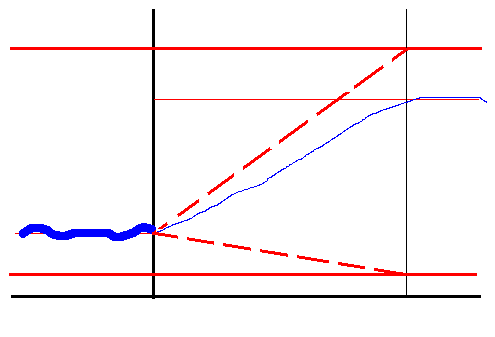
\includegraphics[width=\fullwidth]{graph/dmcplusramprate}
  \scalebox{1}{% Graphic for TeX using PGF
% Title: /home/andre/GIT Repos/AHCampher_thesis/diagrams/dmcplusramprate.dia
% Creator: Dia v0.97.1
% CreationDate: Thu Jan  6 16:23:31 2011
% For: andre
% \usepackage{tikz}
% The following commands are not supported in PSTricks at present
% We define them conditionally, so when they are implemented,
% this pgf file will use them.
\ifx\du\undefined
  \newlength{\du}
\fi
\setlength{\du}{15\unitlength}
\begin{tikzpicture}
\pgftransformxscale{1.000000}
\pgftransformyscale{-1.000000}
\definecolor{dialinecolor}{rgb}{0.000000, 0.000000, 0.000000}
\pgfsetstrokecolor{dialinecolor}
\definecolor{dialinecolor}{rgb}{1.000000, 1.000000, 1.000000}
\pgfsetfillcolor{dialinecolor}
\pgfsetlinewidth{0.050000\du}
\pgfsetdash{}{0pt}
\pgfsetdash{}{0pt}
\pgfsetbuttcap
{
\definecolor{dialinecolor}{rgb}{0.000000, 0.000000, 0.000000}
\pgfsetfillcolor{dialinecolor}
% was here!!!
\definecolor{dialinecolor}{rgb}{0.000000, 0.000000, 0.000000}
\pgfsetstrokecolor{dialinecolor}
\draw (10.000000\du,15.000000\du)--(33.000000\du,15.000000\du);
}
\pgfsetlinewidth{0.050000\du}
\pgfsetdash{}{0pt}
\pgfsetdash{}{0pt}
\pgfsetbuttcap
{
\definecolor{dialinecolor}{rgb}{0.000000, 0.000000, 0.000000}
\pgfsetfillcolor{dialinecolor}
% was here!!!
\definecolor{dialinecolor}{rgb}{0.000000, 0.000000, 0.000000}
\pgfsetstrokecolor{dialinecolor}
\draw (16.000000\du,3.000000\du)--(16.000000\du,15.000000\du);
}
\pgfsetlinewidth{0.150000\du}
\pgfsetdash{}{0pt}
\pgfsetdash{}{0pt}
\pgfsetbuttcap
{
\definecolor{dialinecolor}{rgb}{0.588235, 0.588235, 0.588235}
\pgfsetfillcolor{dialinecolor}
% was here!!!
\definecolor{dialinecolor}{rgb}{0.588235, 0.588235, 0.588235}
\pgfsetstrokecolor{dialinecolor}
\draw (33.000000\du,3.500000\du)--(10.000000\du,3.500000\du);
}
\pgfsetlinewidth{0.150000\du}
\pgfsetdash{}{0pt}
\pgfsetdash{}{0pt}
\pgfsetbuttcap
{
\definecolor{dialinecolor}{rgb}{0.588235, 0.588235, 0.588235}
\pgfsetfillcolor{dialinecolor}
% was here!!!
\definecolor{dialinecolor}{rgb}{0.588235, 0.588235, 0.588235}
\pgfsetstrokecolor{dialinecolor}
\draw (33.000000\du,14.000000\du)--(10.000000\du,14.000000\du);
}
% setfont left to latex
\definecolor{dialinecolor}{rgb}{0.000000, 0.000000, 0.000000}
\pgfsetstrokecolor{dialinecolor}
\node[anchor=west] at (19.000000\du,15.500000\du){Time};
\pgfsetlinewidth{0.050000\du}
\pgfsetdash{}{0pt}
\pgfsetdash{}{0pt}
\pgfsetbuttcap
{
\definecolor{dialinecolor}{rgb}{0.588235, 0.588235, 0.588235}
\pgfsetfillcolor{dialinecolor}
% was here!!!
\definecolor{dialinecolor}{rgb}{0.588235, 0.588235, 0.588235}
\pgfsetstrokecolor{dialinecolor}
\draw (30.000000\du,3.000000\du)--(30.000000\du,15.000000\du);
}
\pgfsetlinewidth{0.200000\du}
\pgfsetdash{{\pgflinewidth}{0.040000\du}}{0cm}
\pgfsetdash{{\pgflinewidth}{0.300000\du}}{0cm}
\pgfsetbuttcap
{
\definecolor{dialinecolor}{rgb}{0.000000, 0.000000, 0.000000}
\pgfsetfillcolor{dialinecolor}
% was here!!!
\definecolor{dialinecolor}{rgb}{0.000000, 0.000000, 0.000000}
\pgfsetstrokecolor{dialinecolor}
\draw (16.000000\du,6.000000\du)--(33.000000\du,6.000000\du);
}
\pgfsetlinewidth{0.200000\du}
\pgfsetdash{{1.500000\du}{1.500000\du}}{0\du}
\pgfsetdash{{0.700000\du}{0.700000\du}}{0\du}
\pgfsetbuttcap
{
\definecolor{dialinecolor}{rgb}{0.000000, 0.000000, 0.000000}
\pgfsetfillcolor{dialinecolor}
% was here!!!
\definecolor{dialinecolor}{rgb}{0.000000, 0.000000, 0.000000}
\pgfsetstrokecolor{dialinecolor}
\draw (16.000000\du,12.000000\du)--(30.000000\du,3.500000\du);
}
\pgfsetlinewidth{0.200000\du}
\pgfsetdash{{0.700000\du}{0.700000\du}}{0\du}
\pgfsetdash{{0.700000\du}{0.700000\du}}{0\du}
\pgfsetbuttcap
{
\definecolor{dialinecolor}{rgb}{0.000000, 0.000000, 0.000000}
\pgfsetfillcolor{dialinecolor}
% was here!!!
\definecolor{dialinecolor}{rgb}{0.000000, 0.000000, 0.000000}
\pgfsetstrokecolor{dialinecolor}
\draw (16.000000\du,12.000000\du)--(30.000000\du,14.000000\du);
}
\pgfsetlinewidth{0.100000\du}
\pgfsetdash{}{0pt}
\pgfsetdash{}{0pt}
\pgfsetmiterjoin
\pgfsetbuttcap
{
\definecolor{dialinecolor}{rgb}{0.000000, 0.000000, 0.000000}
\pgfsetfillcolor{dialinecolor}
% was here!!!
\definecolor{dialinecolor}{rgb}{0.000000, 0.000000, 0.000000}
\pgfsetstrokecolor{dialinecolor}
\pgfpathmoveto{\pgfpoint{10.000000\du}{12.000000\du}}
\pgfpathcurveto{\pgfpoint{11.500000\du}{12.000000\du}}{\pgfpoint{11.000000\du}{11.500000\du}}{\pgfpoint{12.000000\du}{12.000000\du}}
\pgfpathcurveto{\pgfpoint{13.000000\du}{12.500000\du}}{\pgfpoint{13.016650\du}{12.007292\du}}{\pgfpoint{14.000000\du}{12.000000\du}}
\pgfpathcurveto{\pgfpoint{14.983350\du}{11.992708\du}}{\pgfpoint{14.300200\du}{12.412500\du}}{\pgfpoint{15.900100\du}{11.956250\du}}
\pgfpathcurveto{\pgfpoint{17.500000\du}{11.500000\du}}{\pgfpoint{15.750000\du}{11.833333\du}}{\pgfpoint{17.500000\du}{11.500000\du}}
\pgfpathcurveto{\pgfpoint{19.250000\du}{11.166667\du}}{\pgfpoint{18.083333\du}{10.666667\du}}{\pgfpoint{20.500000\du}{10.000000\du}}
\pgfpathcurveto{\pgfpoint{22.916667\du}{9.333333\du}}{\pgfpoint{20.750000\du}{9.000000\du}}{\pgfpoint{24.500000\du}{8.000000\du}}
\pgfpathcurveto{\pgfpoint{28.250000\du}{7.000000\du}}{\pgfpoint{25.030000\du}{6.000000\du}}{\pgfpoint{32.500000\du}{6.000000\du}}
\pgfusepath{stroke}
}
% setfont left to latex
\definecolor{dialinecolor}{rgb}{0.000000, 0.000000, 0.000000}
\pgfsetstrokecolor{dialinecolor}
\node[anchor=west] at (13.000000\du,11.2500000\du){$y(t)$};
% setfont left to latex
\definecolor{dialinecolor}{rgb}{0.000000, 0.000000, 0.000000}
\pgfsetstrokecolor{dialinecolor}
\node[anchor=west] at (10.000000\du,4.25000000\du){High limit};
% setfont left to latex
\definecolor{dialinecolor}{rgb}{0.000000, 0.000000, 0.000000}
\pgfsetstrokecolor{dialinecolor}
\node[anchor=west] at (10.000000\du,14.500000\du){Low limit};
% setfont left to latex
\definecolor{dialinecolor}{rgb}{0.000000, 0.000000, 0.000000}
\pgfsetstrokecolor{dialinecolor}
\node[anchor=west] at (16.000000\du,6.7500000\du){New setpoint};
% setfont left to latex
\definecolor{dialinecolor}{rgb}{0.000000, 0.000000, 0.000000}
\pgfsetstrokecolor{dialinecolor}
\node[anchor=west] at (29.500000\du,15.500000\du){$t_{ss}$};
\end{tikzpicture}
}  
  \caption[DMCplus ramp rate dynamic constraints]{Ramp rates creating dynamic constraints on integrating variables after setpoint change.}
  \label{fig:dmcplusramprates}
\end{figure}

\subsubsection{Interfaces}
The DMCplus Model (figure~\ref{fig:ssdmcplusmodel}) interface is used to obtain models from data.
Obtaining a gain matrix is possible from this interface.
Additions to the model matrix are also made from this interface.

The controller is built using the DMCplus Build interface (figure~\ref{fig:ssdmcpluscontrolbuild}).
Models obtained in the previous step are implemented and a configuration file for the controller is generated.

The Production Control Web Interface (figure~\ref{fig:ssdmcplusoperator}) is used by operators to interact with the process.
This interface is used to change constraints on inputs and outputs during process operation.


% Local Variables:
% TeX-master: "AHC_thesis"
% End:
